\section{Methodology}
\lhead{\leftmark}
The equipment needed and procedures undertaken to carry out CNC Machining are described in the following sections. The experiment was done at ENW-04 (Machine Shop) at the JKUAT Workshops.
\subsection{Equipment}
\begin{enumerate}
\item CNC Machine (available at ENW04 - Machine Shop)
\item Workpiece design as specified by the manual
\item CNC Machine controller (Siemens Sinumerik 828D)
\item Workpiece - Aluminium block 
\end{enumerate}
\begin{figure}[h!]
	\centering
	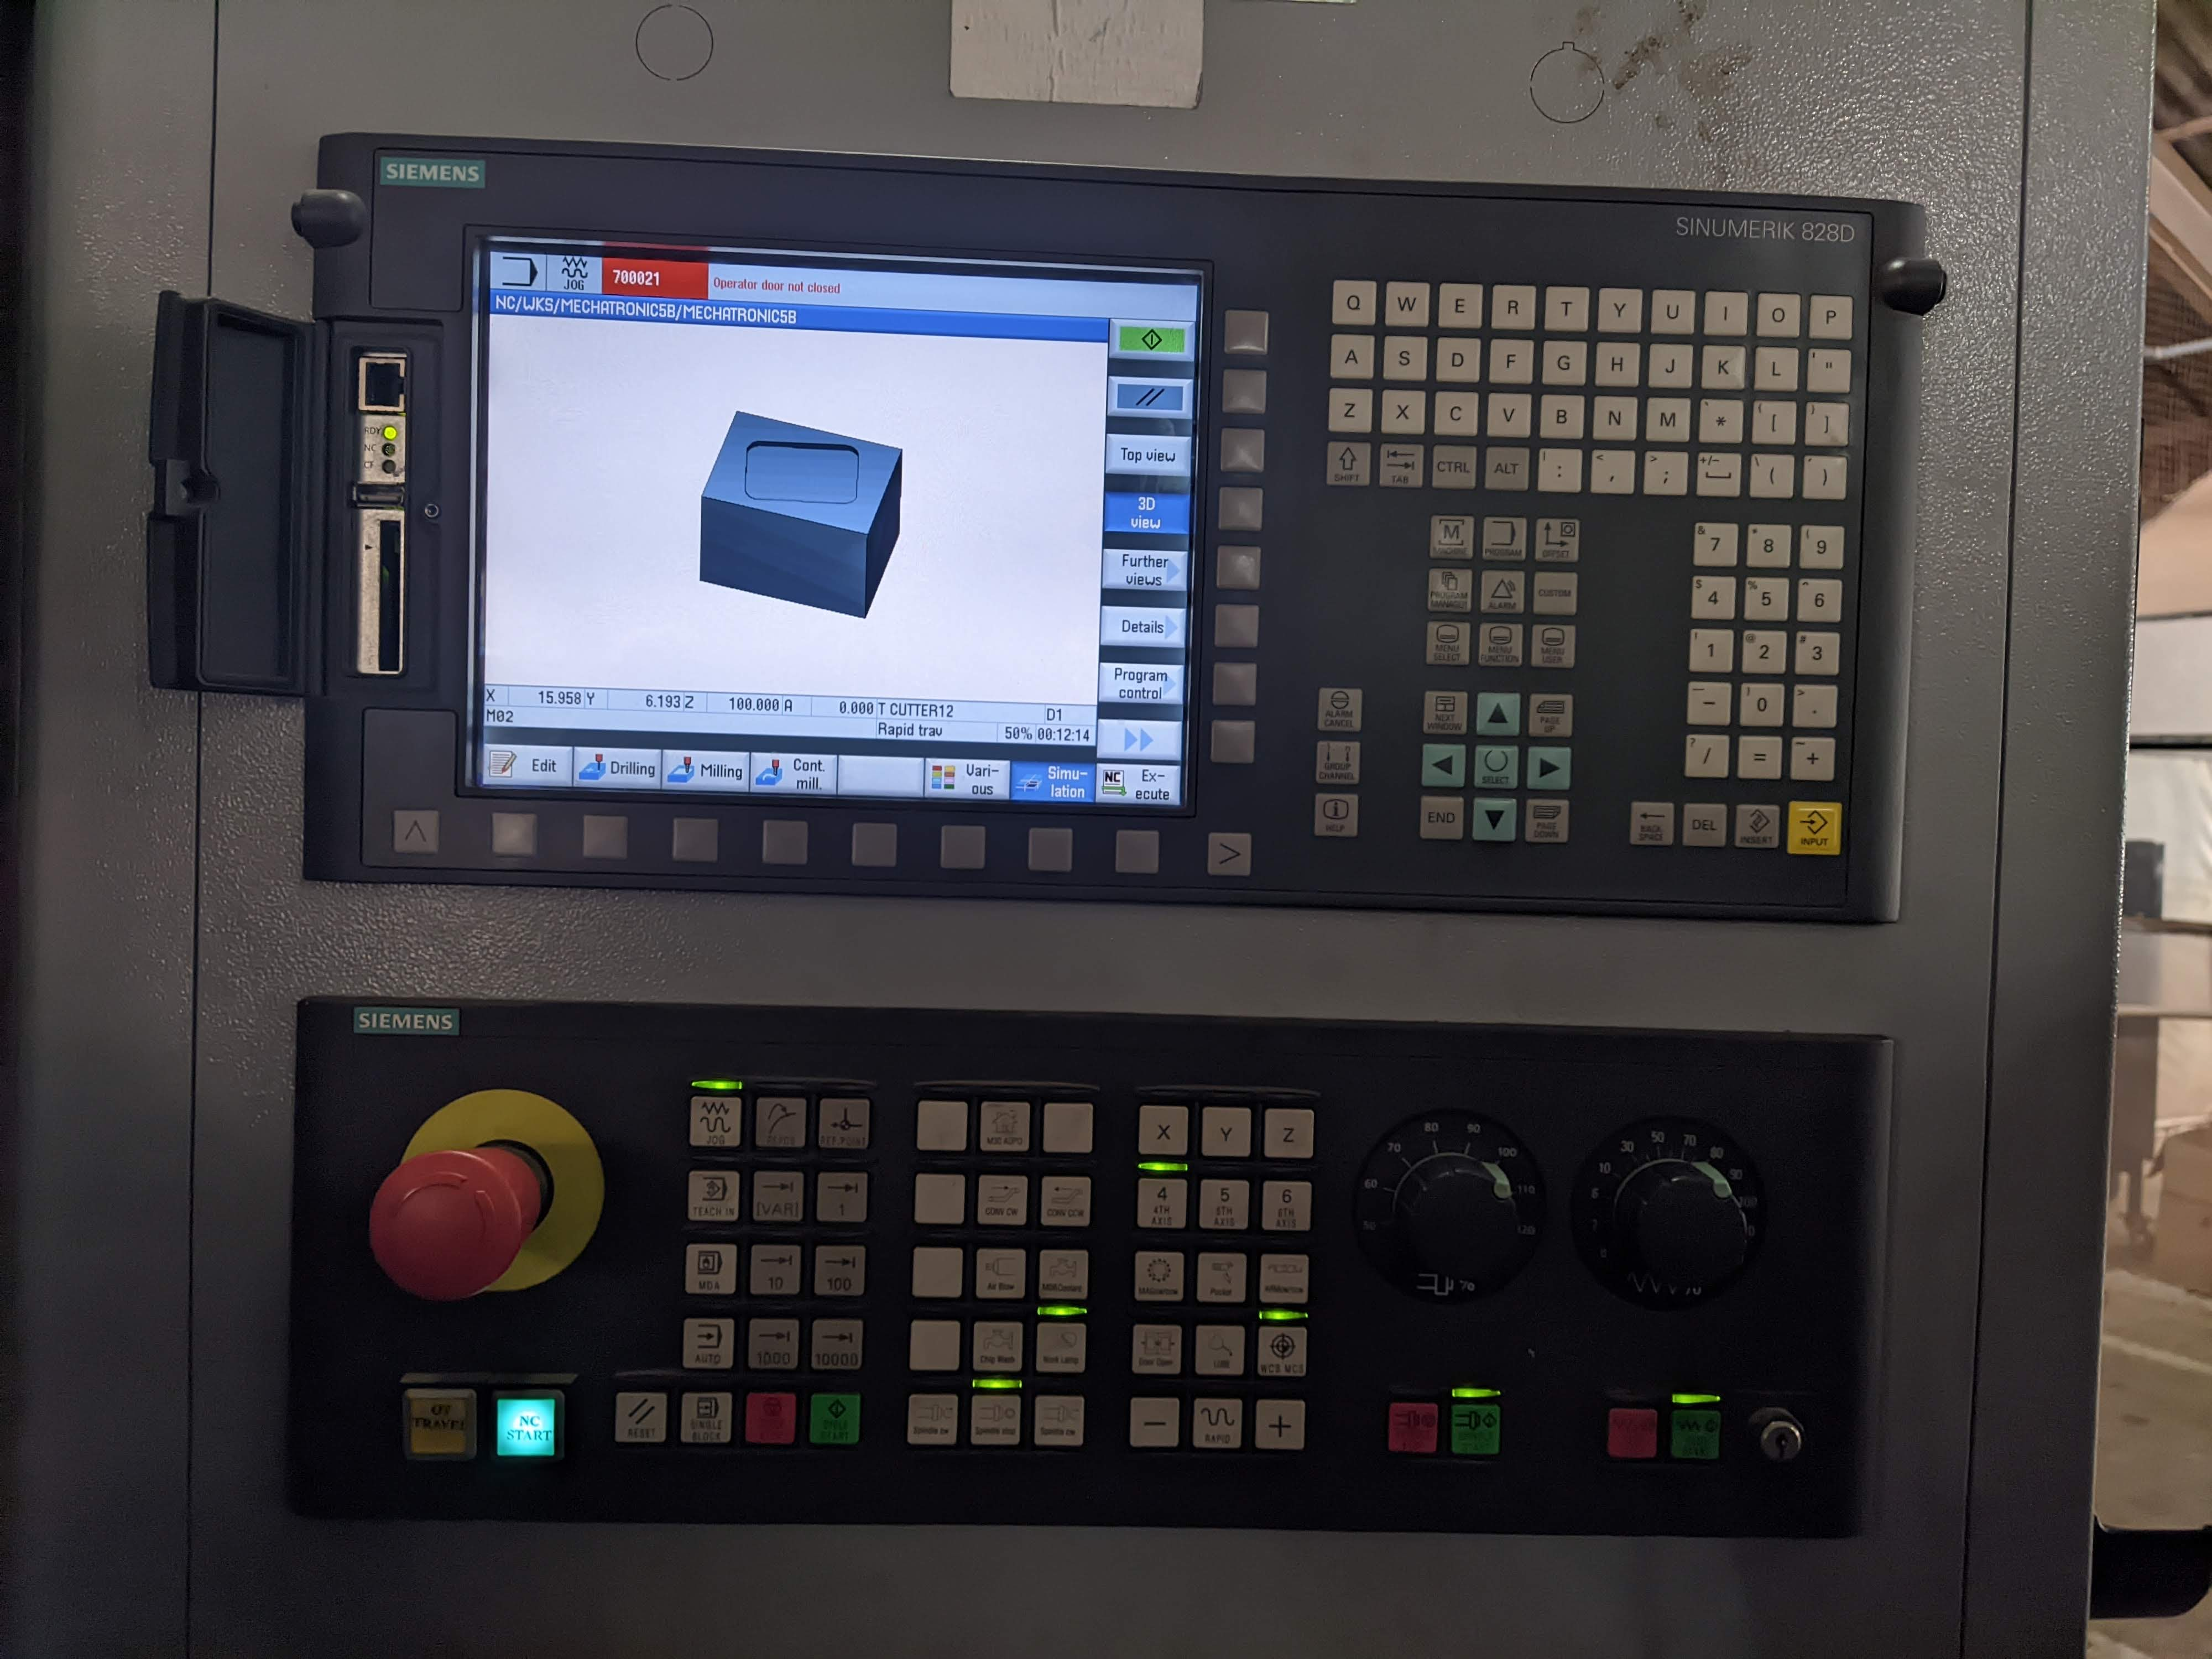
\includegraphics[width=0.7\linewidth]{Figures/machinecontroller}
	\caption[CNC Machine Controller]{CNC Machine Controller - Siemens SINUMERIK\textsuperscript\textregistered 828D} 
	\label{fig:cnccontroller}
\end{figure}
\subsection{Procedure}
Prior to beginning the machining operation, the machine has to be checked for the required items for its functionality, namely:
\begin{enumerate}
	\item Oil - This is necessary for lubrication and is contained in an oil tank at the back of the machine.
	\item Air - the pneumatic system is used by the tool change mechanism, and is supplied via high-pressure pipes and air ducts from an air compressor.
	\item Electricity - 3-$\phi$ electricity is required for the machine drives to move the various actuators along their respective axes.
\end{enumerate}
The operation chosen was a face milling operation to obtain a flat surface, followed by creation of a pocket at an angle of 15\textdegree \space to the horizontal.\\
The shape to be created was analyzed and the dimensions obtained. A tool-path was created using G codes to control the CNC Machine. The codes were programmed into the CNC Machine via the controller board.\\
The workpiece blank was measured to obtain the dimensions, which were programmed into the CNC program. The face milling operation was programmed first, followed by the contouring operation to create the pocket. As the CNC machine is able to interpolate most machining operations internally, for most operations the inputs required are the location of the features as well as their dimensions.\\
Before beginning the machining operation, a simulation was carried out to ascertain that the program was correctly written, with a visual aid of the tool-paths and the features to be created from the stock billet. This step is essential as it enables the operator to catch mistakes and correct them in the program before it has began executing.\\
Some machining parameters such as the speed, feed and use of cutting fluids are chosen based on a handbook provided for different materials. In this case, a spindle speed of 2000rpm and a feed of 150mm/min were chosen, as well as coolant on in flood mode.\\
Machining process once started is carried out to completion unless stopped by an emergency stop button press or the process cancel button in the user interface. Tool changes are done automatically, with the machine stopping the spindle and using pneumatic actuators, the current loaded tool is placed back in the magazine and the tool required for the next operation is automatically loaded.\\
The machining time depends on the  size of the workpiece and the operations being carried out, as well as the cutting speed and feed. Roughing operations were chosen to remove the bulk of the material before carrying out fine machining to achieve the desired surface finish.\\
Once the machining process was completed, the CNC hatch was opened. and the workpiece retrieved for examination.
\begin{figure}[h!]
	\centering
	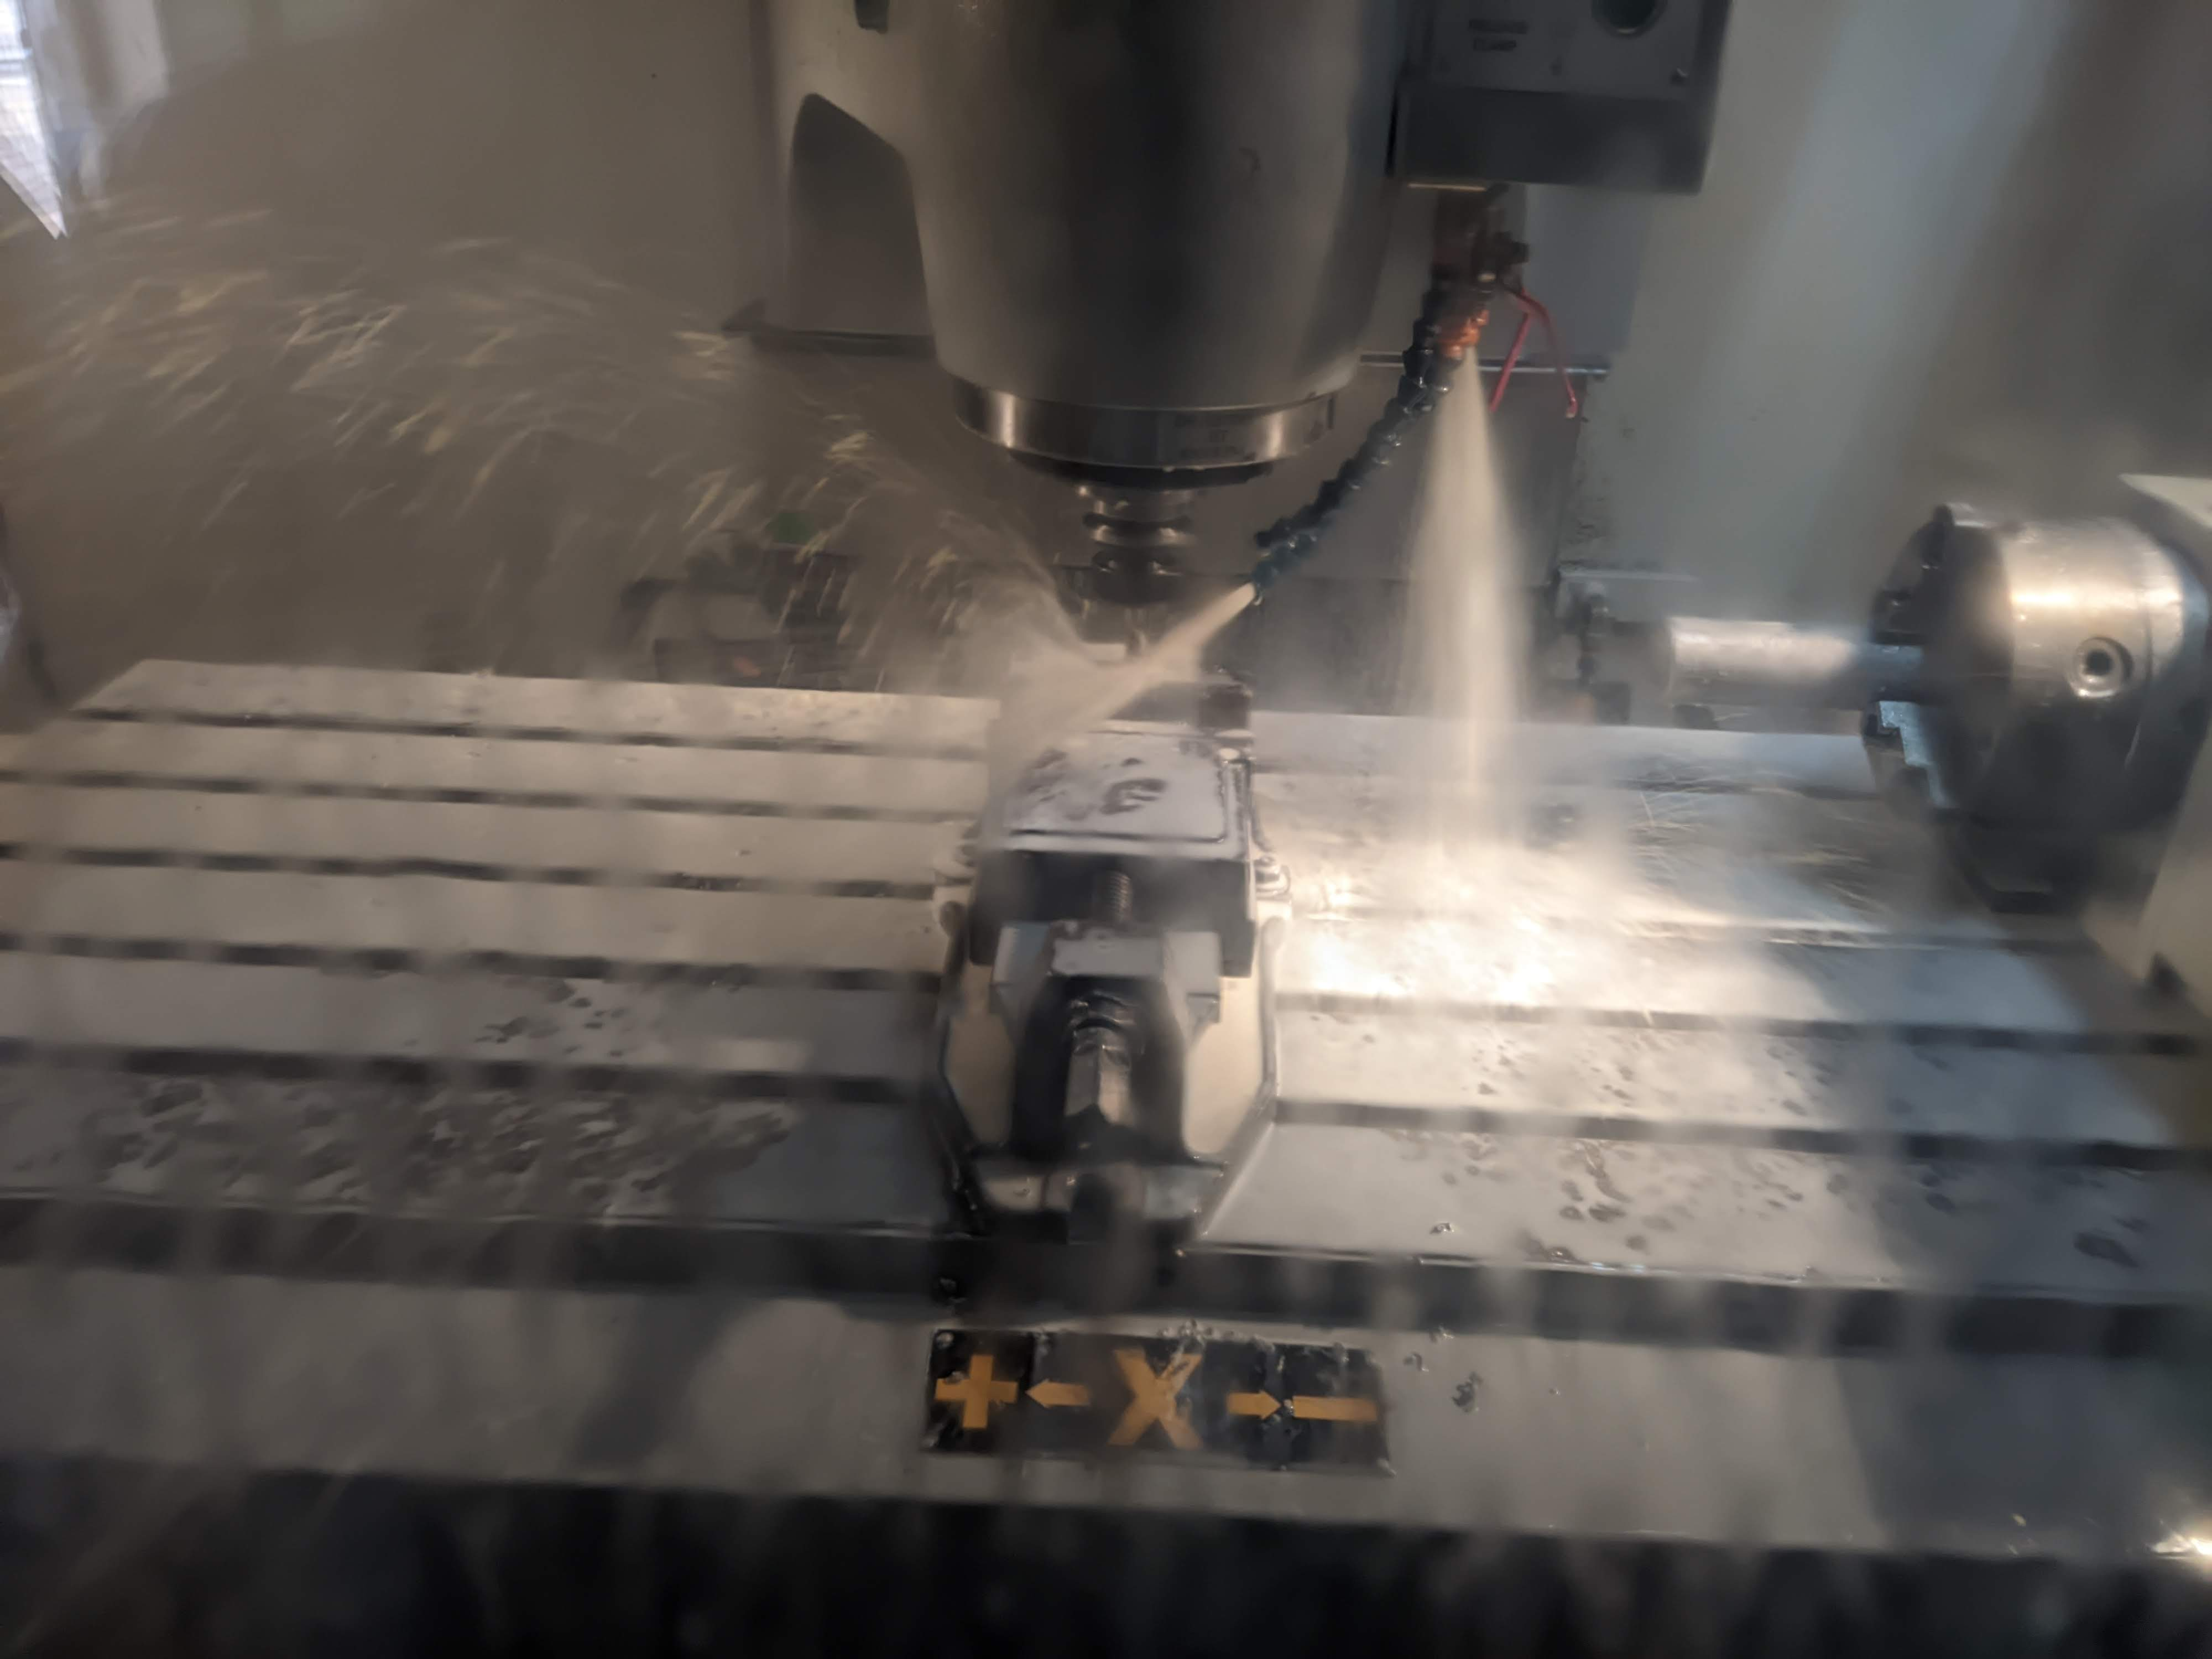
\includegraphics[width=0.8\linewidth]{Figures/machining}
	\caption[CNC Machining Process]{CNC Machining Process Underway}
	\label{fig:machining}
\end{figure}
%\begin{verbatim}
%	G21
%	G92 X0.0 Y0.0
%	S1D1
%	G01 X7.0 Y0.0
%	G01 X0.0 Y-7.0
%	G01 X-7.0 Y0.0
%	G00 X0.0 Y0.0
%	M02
%\end{verbatim}